\documentclass[11pt,a4paper]{article}

\usepackage[utf8]{inputenc}
\usepackage[T1]{fontenc}
\usepackage[margin=1in]{geometry}
\usepackage{amsmath,amssymb}
\usepackage{graphicx}
\usepackage{booktabs}
\usepackage{multirow}
\usepackage{hyperref}
\usepackage{xcolor}
\usepackage{enumitem}
\usepackage{caption}
\usepackage{subcaption}
\usepackage{algorithm}
\usepackage{algpseudocode}
\usepackage{tikz}
\usetikzlibrary{shapes.geometric, arrows.meta, positioning, fit, backgrounds}
\usepackage{natbib}
\bibliographystyle{plainnat}

\hypersetup{
    colorlinks=true,
    linkcolor=blue!60!black,
    citecolor=blue!60!black,
    urlcolor=blue!60!black
}

\title{Model as Reader: Matching Frontier LLM Accuracy with Small Open-Source Models via Deterministic Orchestration and Graph-Structured Retrieval}

\author{Manoj M\\Independent Researcher\\\texttt{manoj.manoharan.dev@gmail.com}}

\date{June 2026}

\begin{document}

\maketitle

% ============================================================
\begin{abstract}
We present an architecture in which a small on-device language model (8B parameters) matches or exceeds a frontier model (Claude Sonnet) on multi-hop structured knowledge retrieval, not by improving the model, but by reducing its job. A deterministic orchestrator decomposes complex queries, a temporal knowledge graph handles multi-hop traversal, and the model's only task is reading 2--20 pre-selected facts and producing one answer. Across three experimental phases---architecture validation with a frontier model, local model validation with Llama 3.1 8B, and a 26-test capability profiling harness run across four models---we find that (1) the orchestrated 8B model scores 13/13 on our benchmark versus Sonnet's 12/13, reading 5.5\% of the corpus, (2) every failure across all phases traced to orchestrator code bugs, never to model comprehension, and (3) model capability tiers determine where the code/model boundary should be drawn, not whether the architecture works. These results are demonstrated on a synthetic 200-fact corpus with 13 multi-hop questions. We present them as preliminary evidence for a position: that small models are underexplored as components in hybrid systems because evaluation practices conflate model capability with system capability, and that the distribution of cognitive labor between code and model is the primary design variable.
\end{abstract}

% ============================================================
\section{Introduction}
\label{sec:intro}

The dominant framing in language model research treats accuracy as a property of the model. A harder question demands a larger model. Multi-hop reasoning requires a model that can reason across multiple hops. This framing is so pervasive that ``scaling up'' has become the default response to capability gaps.

We propose an alternative: for structured knowledge retrieval tasks, accuracy is a property of the \emph{system}, not the model. A small model embedded in the right architecture can match a frontier model, because the hard parts of the task---decomposition, traversal, retrieval, temporal resolution---are better handled by deterministic code than by probabilistic inference.

The insight is a separation of concerns. Code handles what code is good at: graph traversal, path finding, entity extraction, temporal supersession, working memory management. The model handles what models are good at: reading a small set of pre-selected facts and producing a natural language answer. We call this the \textbf{model-as-reader} architecture.

This is not a new observation in isolation. HippoRAG \citep{gutierrez2024hipporag} uses knowledge graphs to index retrieval. GraphRAG \citep{edge2024graphrag} uses community summaries for global sensemaking. EvoReasoner \citep{evoreasoner2024} matches a 671B model with 8B using temporal knowledge graphs. MemGPT \citep{packer2023memgpt} externalizes memory to an OS-inspired hierarchy. What we contribute is an explicit experimental arc that starts from the thesis, fails instructively, iterates based on evidence, and produces both a validated architecture and a methodology for profiling model capability within that architecture.

We scope the claim carefully. This architecture solves \textbf{entity-relationship queries over structured data with temporal updates}: customer data, project tracking, organizational knowledge, personal CRM, regulatory compliance. Not general reasoning. Not summarization. Not creative work. Within this scope, we present evidence that the approach works, characterize where it breaks, and identify what remains open.

The results are demonstrated on a synthetic corpus. We are explicit about this limitation throughout.

% ============================================================
\section{Architecture}
\label{sec:arch}

\subsection{Design Principles}

The architecture rests on three principles derived from experimental failure (Section~\ref{sec:phase1}):

\begin{enumerate}[leftmargin=*]
    \item \textbf{Memory as routing index, not accumulator.} Our first experiment loaded all facts through the model in batches, re-sending a memory JSON every step. This used 5--13$\times$ more tokens for identical accuracy. The correct role for memory is directing the model to minimal, pre-selected context.

    \item \textbf{Path-edge retrieval, not entity-fact retrieval.} Retrieving all facts about entities on a graph path produces 33+ facts per query (bloat). Retrieving only the facts that \emph{connect} entities along the path produces 4--8 facts. The difference is the gap between 62\% and 92\% accuracy in our experiments.

    \item \textbf{The model is the reader, never the planner.} The model never decides what to retrieve, how to decompose a query, or which path to traverse. It reads facts and answers questions. One hop. One answer.
\end{enumerate}

\subsection{System Components}

The system consists of four components (Figure~\ref{fig:arch}):

\textbf{Temporal Knowledge Graph (persistent).} Entity nodes with versioned properties. Relationship edges with timestamps. New edges auto-close previous values (temporal supersession). Implemented as an adjacency list with per-entity fact indices.

\textbf{Deterministic Orchestrator (stateless per query).} Classifies the query type (direct lookup, override/temporal, chain, connection, aggregation). Extracts entities via string matching. Selects a retrieval strategy: multi-path DFS for connection queries, entity-fact lookup for direct/override, 1-hop neighbor expansion for chain queries, pattern matching for aggregation. Retrieves only path-edge facts. Feeds the minimal fact set to the model.

\textbf{Working Memory (per-task, ephemeral).} A JSON object tracking the current goal, resolved sub-answers, and pending steps. Used only in step-by-step mode. Discarded after task completion. In practice, the single-call path retrieval mode outperformed step-by-step on all conditions tested.

\textbf{Small Model (on-device).} Receives 2--20 facts and one question. Produces one answer. Runs locally via Ollama. No API calls, no fine-tuning, no prompt engineering beyond a fixed two-sentence system prompt.

\begin{figure}[t]
\centering
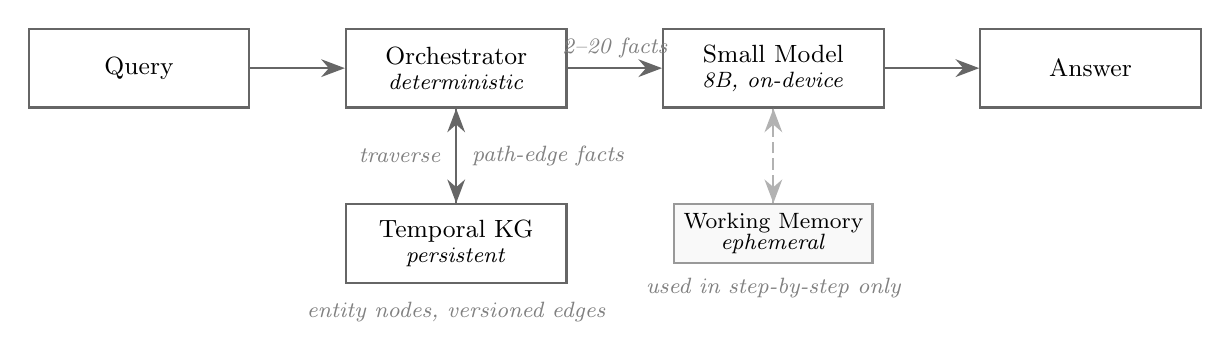
\begin{tikzpicture}[
    node distance=0.8cm and 1.2cm,
    block/.style={rectangle, draw=black!60, fill=white, thick, minimum height=1cm, minimum width=2.8cm, align=center, font=\small},
    smallblock/.style={rectangle, draw=black!40, fill=gray!5, thick, minimum height=0.7cm, minimum width=2.2cm, align=center, font=\footnotesize},
    arrow/.style={-{Stealth[length=3mm]}, thick, black!60},
    label/.style={font=\footnotesize\itshape, text=black!50},
]

% Main flow
\node[block] (query) {Query};
\node[block, right=of query] (orch) {Orchestrator\\[-2pt]\footnotesize\textit{deterministic}};
\node[block, right=of orch] (model) {Small Model\\[-2pt]\footnotesize\textit{8B, on-device}};
\node[block, right=of model] (answer) {Answer};

% KG below orchestrator
\node[block, below=1.2cm of orch] (kg) {Temporal KG\\[-2pt]\footnotesize\textit{persistent}};

% Working memory below model
\node[smallblock, below=1.2cm of model] (wm) {Working Memory\\[-2pt]\footnotesize\textit{ephemeral}};

% Arrows
\draw[arrow] (query) -- (orch);
\draw[arrow] (orch) -- node[above, label] {2--20 facts} (model);
\draw[arrow] (model) -- (answer);
\draw[arrow] (orch) -- node[left, label, xshift=-2pt] {traverse} (kg);
\draw[arrow] (kg) -- node[right, label, xshift=2pt] {path-edge facts} (orch);
\draw[arrow, dashed, black!30] (model) -- (wm);
\draw[arrow, dashed, black!30] (wm) -- (model);

% Annotations
\node[label, below=0.1cm of kg] {entity nodes, versioned edges};
\node[label, below=0.05cm of wm] {used in step-by-step only};

\end{tikzpicture}
\caption{Model-as-reader architecture. The orchestrator handles query classification, entity extraction, graph traversal, and fact selection. The model receives only path-edge facts (typically 4--14 out of 200) and produces a single answer. Dashed lines indicate the working memory path, used only in step-by-step mode.}
\label{fig:arch}
\end{figure}

\subsection{Retrieval Strategies}

Query classification determines the retrieval strategy:

\begin{itemize}[leftmargin=*]
    \item \textbf{Connection queries} (``Trace the chain from X to Y''): Multi-path DFS finds all paths between extracted entities up to 5 hops. Only path-edge facts are retrieved. This is the critical strategy for multi-hop questions.

    \item \textbf{Override queries} (``What is the current budget of X?''): Entity-fact lookup retrieves all facts mentioning the entity. The model sees multiple temporal values and selects the latest. At scale, code-side temporal sorting is more reliable (Section~\ref{sec:phase3}).

    \item \textbf{Chain queries} (``What is X's husband's job?''): 1-hop neighbor expansion from seed entities, retrieving facts for all neighbors.

    \item \textbf{Aggregation queries} (``How many companies were acquired?''): Pattern matching (regex for ``acquired'') across all facts.

    \item \textbf{Direct queries} (``Who is the CEO of X?''): Entity-fact lookup.
\end{itemize}

The classification itself is deterministic: regex patterns over the query text. This is deliberately simple. It works at the current benchmark scale. It will not generalize to unconstrained natural language without a learned classifier, which we note as a limitation.

% ============================================================
\section{Experimental Setup}
\label{sec:setup}

\subsection{Corpus}

A synthetic tech ecosystem corpus at three scales: 60, 120, and 200 facts. 15 companies, approximately 35 named individuals, with roles, marriages, sibling relationships, corporate acquisitions, strategic partnerships, products, project budgets with multiple temporal overrides, and leadership changes with reversals. At the 200-fact scale, approximately 80 facts are structurally meaningful and 120 are noise (company announcements, office updates). Noise facts share entity mentions with core facts, ensuring that retrieval methods must discriminate.

The knowledge graph at 200 facts contains 54 entity nodes. Entity types include persons, companies, and projects. Relationships include employment, family (marriage, siblings, parent-child), corporate (acquisition, partnership, investment), and project membership.

\subsection{Benchmark Questions}

13 questions at the 200-fact scale: 3 direct lookup, 3 temporal override (including a leadership reversal), 2 two-hop chains, 2 three-hop chains requiring traversal across personal and corporate relationships, 2 four-hop chains, and 1 aggregation. Ground truth is verified. Multi-hop chains require 3--5 hops through a mix of personal relationships (marriage, siblings) and corporate relationships (employment, acquisition).

Automated checking uses regex patterns with manual verification of edge cases. Two valid answer chains are accepted for questions with multiple valid paths.

\subsection{Models Tested}

Phase 1: Claude Sonnet (via API, in-browser). Phase 2: Llama 3.1 8B and Gemma 2 2B (via Ollama, local). Phase 3: Llama 3.1 8B, Gemma 2 2B, DeepSeek V4 Pro, and DeepSeek V4 Flash (Ollama for local models, OpenAI-compatible API for DeepSeek).

No model was fine-tuned. All models used the same fixed system prompt: ``Answer precisely based only on provided information.'' No prompt engineering was performed beyond this.

% ============================================================
\section{Phase 1: Architecture Validation}
\label{sec:phase1}

Phase 1 ran three experiments as React browser artifacts calling the Anthropic API, all using Claude Sonnet.

\subsection{Experiment 1: Memory as Accumulator (Failed)}

We implemented memory as a JSON object updated between steps. The model processed all facts in batches, with the full memory re-sent at each step. On a 12-dimension comparison task, single-shot scored 12/12. Memory conditions used 5--13$\times$ more tokens for identical accuracy.

The task was not hard enough to need memory, and the architecture was wrong: memory duplicated what the model saw rather than reducing it. This failure motivated the routing-index design.

\subsection{Experiment 2: Retrieval Paradigm Comparison}

Four retrieval methods on the 200-fact corpus (Table~\ref{tab:rag}).

\begin{table}[h]
\centering
\caption{Retrieval paradigm comparison at 200 facts (Sonnet).}
\label{tab:rag}
\begin{tabular}{@{}lccc@{}}
\toprule
Method & Accuracy & Facts Seen & Tokens/Q \\
\midrule
Single-shot (all facts) & 12/13 (92\%) & 200 & 6{,}922 \\
Naive RAG (keyword top-K) & 7/13 (54\%) & 15 & 4{,}445 \\
HippoRAG-style BFS (3-hop) & 11/13 (85\%) & 24 & 4{,}587 \\
GraphRAG v2 (community summaries) & 12/13 (92\%) & summaries & 5{,}544 \\
\bottomrule
\end{tabular}
\end{table}

Naive RAG is structurally broken for multi-hop queries: it cannot find intermediate entities absent from the question text. Personalized PageRank (PPR) was tested as an alternative to BFS and performed worse (9/13 vs.\ 11/13). PPR penalizes distance, which is counterproductive on a 54-node graph where correct answers require traversing distant nodes. PPR is designed for graphs at 10K+ nodes where prioritization is necessary.

\subsection{Experiment 3: Deterministic Orchestrator}

Three conditions, all using Sonnet (Table~\ref{tab:phase1}).

\begin{table}[h]
\centering
\caption{Phase 1 orchestrator results at 200 facts (Sonnet).}
\label{tab:phase1}
\begin{tabular}{@{}lccc@{}}
\toprule
Condition & Accuracy & Avg Facts & Tokens/Q \\
\midrule
A: Single Shot & 12/13 (92\%) & 200 & 6{,}919 \\
B: Path Retrieval & 12/13 (92\%) & 11 & 4{,}399 \\
C: Step-by-Step & 12/13 (92\%) & 11 & 11{,}600 \\
\bottomrule
\end{tabular}
\end{table}

Condition B matches A while reading 5.5\% of the corpus and using 36\% fewer tokens. Condition C adds no accuracy over B but costs 2.6$\times$ more tokens. Step-by-step decomposition is unnecessary for Sonnet but exists as the mechanism enabling small models.

\textbf{Bug discovery.} Initial B and C scored 8/13 (62\%). Diagnosis via debug logging---not architectural changes---revealed four bugs: (1)~regex misclassification of possessive forms (e.g., ``Labs' founder''), (2)~BFS shortest-path bias finding corporate shortcuts instead of personal chains, (3)~context fact bloat pulling all facts about path entities (33+ facts) instead of path-edge facts (4--8), (4)~overly narrow ground truth accepting only one valid chain when two existed. All four were code bugs. None required prompt changes or model changes.

% ============================================================
\section{Phase 2: Local Model Validation}
\label{sec:phase2}

Phase 2 ran the same benchmark locally via Ollama against Llama 3.1 8B and Gemma 2 2B (Table~\ref{tab:phase2}).

\begin{table}[h]
\centering
\caption{Phase 2 results at 200 facts.}
\label{tab:phase2}
\begin{tabular}{@{}lccc@{}}
\toprule
Condition & Accuracy & Stable & Facts Seen \\
\midrule
8B orchestrated & 13/13 & Yes & $\sim$14 \\
8B single-shot & 11--12/13 & No & 200 \\
2B orchestrated & 12--13/13 & No & $\sim$14 \\
Sonnet orchestrated (Phase 1) & 12/13 & Yes & 11 \\
\bottomrule
\end{tabular}
\end{table}

The orchestrated 8B model scored 13/13, exceeding Sonnet's 12/13. Two additional code bugs were found: (1)~DFS terminated at target entities without expanding to connected persons, and (2)~endpoint expansion was directional and depended on Python \texttt{set()} hash randomization, causing intermittent failures across process invocations. Both were fixed in the orchestrator. Neither required any change to the model or its prompt.

Gemma 2B achieved 13/13 on three of five runs but failed intermittently on one question due to noise fact bloat from endpoint expansion (29 facts instead of 4--5), causing the model to produce a plausible but incorrect reasoning chain.

\textbf{Observation.} Orchestration helps small models more than large ones. Sonnet gained efficiency (36\% fewer tokens) but no accuracy. The 8B model gained both accuracy (+1 to +2 points, depending on single-shot run) and stability (eliminated rotating failures). This is consistent with the thesis that the architecture matters more as model capability decreases.

% ============================================================
\section{Phase 3: Capability Profiling}
\label{sec:phase3}

The 13-question benchmark was saturated: it could not discriminate between Gemma 2B, Llama 8B, and Sonnet as readers. A finer instrument was needed.

\subsection{Harness Design}

We built a 26-test automated harness producing 1{,}560 trials (26 tests $\times$ 3 difficulty levels $\times$ 20 trials per cell). Each test is a self-contained generator and checker. Every trial is deterministic (seeded). Results are stored in append-only JSONL with versioned folders, enabling resume on restart. Four judgment bins: correct, abstained, confident\_wrong, and format\_error. Confident\_wrong is the critical metric.

Test taxonomy is decoupled from test implementation: grouping is an analysis-time concern defined in separate taxonomy files. Adding a new test requires one generator file and one import statement. Zero changes to the harness runner.

\subsection{Test Dimensions}

The 26 tests span five areas:

\textbf{Locate} (3 tests): simple extraction, distractor density, position bias.

\textbf{Match} (2 tests): paraphrase recognition, similar-name discrimination.

\textbf{Reason} (6 tests): negation, absence detection, temporal ordering, comparison, counting, two-hop transitivity.

\textbf{Ingestion} (3 tests): entity extraction from text, relationship triple extraction, supersession detection.

\textbf{Load-bearing single-fact comprehension} (12 tests): surface form variation, question form variation, multi-info extraction, negation in facts, numeric precision, temporal precision, domain-specific language, minimal pairs, instruction adherence (fact contradicts world knowledge), embedded corrections, conditional vs.\ asserted facts, quoted attribution.

\subsection{Results}

Three capability tiers emerged across four models (Table~\ref{tab:tiers}).

\begin{table}[h]
\centering
\caption{Capability tiers across model sizes. Accuracy ranges reflect variation across difficulty levels.}
\label{tab:tiers}
\begin{tabular}{@{}llccc@{}}
\toprule
Tier & Dimension & Gemma 2B & Llama 8B & Frontier \\
\midrule
\multirow{3}{*}{1 (all reliable)} & Locate/Match & $\sim$98\% & 100\% & 100\% \\
 & Fact extraction & 85--100\% & 95--100\% & 100\% \\
 & Supersession detection & 90\% & 95--98\% & 90--100\% \\
\midrule
\multirow{4}{*}{2 (8B+)} & Negation & 20--45\% & 100\% & 100\% \\
 & Transitivity & 65--85\% & 100\% & 100\% \\
 & Instruction adherence & 50\% & 100\% & 100\% \\
 & Simple counting & 0--15\% & 35--100\% & * \\
\midrule
\multirow{3}{*}{3 (code-side)} & Counting ($\geq$5 items) & 0\% & 35\% & * \\
 & Temporal ordering ($\geq$4) & 30--55\% & 65--75\% & 100\% \\
 & Conditional reasoning & broken & 55--90\% & * \\
\bottomrule
\end{tabular}
\vspace{2pt}
\raggedright\footnotesize * Frontier model correctly refuses to assert from potentially incomplete fact sets. Fixable with prompt-level completeness framing.
\end{table}

\textbf{Tier 1} (all models reliable): locate, match, entity extraction, simple extraction, embedded correction. Safe to delegate to any model.

\textbf{Tier 2} (8B reliable, 2B broken): negation, counting on small sets, transitivity, absence detection, explicit relationship extraction, instruction adherence. The jump from 2B to 8B fixes these dimensions.

\textbf{Tier 3} (neither small model reliable): counting at 5+ items, temporal ordering at 4+ updates, implicit relationship extraction, conditional/epistemic reasoning. These require code-side solutions regardless of model size.

A fourth model, DeepSeek V4 Flash, was tested but showed a meaningful capability gap relative to V4 Pro, confirming that ``frontier'' is not a uniform category. Flash results are omitted from the tier table for clarity; V4 Pro represents the frontier ceiling.

\subsection{Frontier Epistemic Strictness}

An unexpected finding: frontier models (DeepSeek V4 Pro) are epistemically stricter than small models. When given a fact set stating that two people work at a company and asked ``how many people work there?'', the frontier model correctly reasons that two listed people does not imply two total people, and refuses to assert. Small models assume completeness without being told, producing the ``correct'' answer for the wrong reason.

This is not a bug in either model. It reflects a different epistemic contract. The implication for system design: frontier models need prompts establishing fact completeness (``the following facts are the complete set''); small models need code-side guardrails against overconfident wrong answers.

\subsection{Code-Solvable Failures}

Every Tier 3 failure identified has a deterministic code-side fix:

\begin{table}[h]
\centering
\caption{Tier 3 failures and their code-side solutions.}
\label{tab:codefixes}
\begin{tabular}{@{}ll@{}}
\toprule
Failure & Code Fix \\
\midrule
Counting at scale & \texttt{len(filtered\_list)} in orchestrator \\
Temporal ordering at scale & Sort by timestamp, give model only latest \\
Negation (2B) & Positive extraction, code computes complement \\
Absence detection & Code checks set membership \\
Conditional statements & Regex filter for hedging language pre-model \\
Implicit relationships & Pattern matching for ``left X to join Y'' \\
\bottomrule
\end{tabular}
\end{table}

This reinforces the core thesis: the model's role is reading pre-selected facts, and every failure outside that role is better handled by code.

% ============================================================
\section{Discussion}
\label{sec:discussion}

\subsection{All Bugs Were Code Bugs}

Across three phases and hundreds of trials, no failure traced to model comprehension. The failures were: regex misclassification, BFS shortest-path bias, context fact bloat, ground truth too narrow, DFS endpoint non-expansion, Python set hash randomization, checker regex patterns. Every one was fixed in the orchestrator or test harness. No prompt was changed. No model was fine-tuned.

This is the operational advantage of the model-as-reader architecture. When the model's job is constrained to single-hop extraction from pre-selected context, debugging is software engineering, not prompt engineering. Failures are deterministic and traceable. Root causes are identifiable from logs. Fixes are verifiable.

\subsection{The Code/Model Boundary as Design Variable}

The capability tiers from Phase 3 define where the boundary should be drawn for each model size:

For a \textbf{2B model}: orchestrator handles counting, negation, absence, transitivity, temporal sorting, comparison, relationship extraction, conditional filtering. Model only does simple extraction and entity matching.

For an \textbf{8B model}: orchestrator handles counting at scale, temporal sorting at scale, conditional/epistemic filtering. Model handles everything else.

For a \textbf{frontier API}: fix prompt to establish fact completeness. Model handles everything. But this forfeits privacy, offline operation, zero-latency, and cost predictability.

The tiers themselves suggest a hypothesis about model architecture: capability differences between 2B and 8B may correspond to the number of sequential internal operations (circuit depth) the model can perform. Tier 1 tasks require depth-1 processing (read fact, extract value). Tier 2 tasks require depth-2 (read fact, apply logical operation). Tier 3 tasks require variable-depth iteration (process N items sequentially). This is a synthesized hypothesis, not a verified finding, but it is testable by varying task depth while holding context length constant.

\subsection{Why Small Models Are Underexplored}

Standard benchmarks evaluate models in isolation: give the model a question and a context, measure accuracy. This conflates model capability with system capability. An 8B model scores poorly on multi-hop reasoning benchmarks not because it cannot read facts, but because it cannot plan, decompose, and retrieve simultaneously. If you remove those responsibilities, the reading capability is nearly identical to frontier models.

This observation is not unique to our work. EvoReasoner \citep{evoreasoner2024} demonstrated similar results with temporal knowledge graphs. But the broader implication is underexplored, partly because the incentive structure of model development favors scaling (which is a single-variable intervention) over architectural composition (which requires engineering effort specific to each task category).

% ============================================================
\section{Related Work}
\label{sec:related}

\textbf{Graph-augmented retrieval.} HippoRAG \citep{gutierrez2024hipporag} uses a hippocampus-inspired architecture with knowledge graphs as a retrieval index, achieving 10--30$\times$ cost reduction over iterative retrieval methods. Our work uses a simpler graph structure (adjacency list with DFS) and focuses on the model's role rather than the retrieval algorithm. GraphRAG \citep{edge2024graphrag} uses community detection and LLM-generated summaries for global sensemaking queries. We tested a GraphRAG-inspired approach (community summaries) and found it matched single-shot accuracy but at higher cost than path-edge retrieval.

\textbf{Memory architectures for LLMs.} MemGPT \citep{packer2023memgpt} proposes an OS-inspired memory hierarchy for extending LLM context. Graphiti/Zep \citep{graphiti2025} implements a temporal knowledge graph with incremental updates and a bi-temporal data model. GBrain \citep{gbrain2025} achieves zero-LLM-call graph wiring via regex patterns over markdown. Our two-tier memory (working memory + temporal KG) is architecturally similar to these systems but scoped to the specific question of whether the architecture enables small models to match large ones.

\textbf{Small models matching large ones.} EvoReasoner \citep{evoreasoner2024} demonstrates an 8B model matching a 671B model using temporal knowledge graphs and multi-hop decomposition. Our work arrives at a similar conclusion from a different starting point (engineering-first rather than ML-first) and contributes the capability profiling methodology for characterizing model-specific code/model boundaries.

\textbf{Retrieval-augmented generation.} Standard RAG \citep{lewis2020rag} retrieves documents via embedding similarity. Our experiments confirm that naive keyword-based RAG is structurally broken for multi-hop queries because it cannot locate intermediate entities absent from the question text. Graph-structured retrieval addresses this by following relationship edges rather than matching query terms.

% ============================================================
\section{Limitations}
\label{sec:limitations}

We are explicit about what this work does not establish:

\begin{enumerate}[leftmargin=*]
    \item \textbf{Synthetic benchmark.} All results are on a hand-crafted corpus of 200 facts with 13 questions. We have not tested on established multi-hop QA benchmarks (HotpotQA, MuSiQue, 2WikiMultiHopQA) or real-world data. The corpus is clean by construction: facts are grammatically regular, entities are unambiguous, relationships are explicit. Real-world text (CRM tickets, legal documents, unstructured notes) will be messier.

    \item \textbf{Entity extraction is string matching.} At 200 facts and 35 entities, string matching works. At 1{,}000+ entities with name collisions, partial matches, and coreference, it will break. This is likely the true ceiling of the current implementation.

    \item \textbf{Scale is untested beyond 200 facts.} The noise-to-signal ratio will increase with corpus size. Path-edge retrieval should become relatively more advantageous (the token gap widens), but entity extraction noise will also increase.

    \item \textbf{Statistical rigor is limited.} Phase 2 ran 2--5 repetitions per condition. Phase 3 ran 20 trials per cell. Neither provides strong statistical significance. Confidence intervals are not reported.

    \item \textbf{Query classification is regex-based.} The current classifier handles the 13 benchmark questions but will not generalize to unconstrained natural language without a learned component.

    \item \textbf{No comparison on established benchmarks.} We cite HippoRAG, GraphRAG, and EvoReasoner but do not evaluate on their benchmarks. A direct comparison would strengthen or weaken the claims substantially.
\end{enumerate}

% ============================================================
\section{Open Questions}
\label{sec:open}

\begin{enumerate}[leftmargin=*]
    \item Does the architecture hold at 500+ facts? The token efficiency advantage should increase, but entity extraction noise and graph density may degrade path quality.

    \item Can the same orchestration pattern handle ingestion? Decomposing the write side into single-hop steps (entity extraction, coreference resolution, relationship extraction, supersession detection, verification) is architecturally natural but untested.

    \item Does boolean gate evaluation (facts + predicate $\rightarrow$ true/false) compose reliably? If per-gate accuracy is 95\%, majority voting of three gates yields $\sim$99.3\%. Practical determinism via redundancy, verification gates, and explicit uncertainty boundaries. This is a separate thesis, not yet experimentally validated.

    \item Can fine-tuning close the Tier 3 gaps? The Phase 3 generators produce training data for weak dimensions. LoRA/QLoRA targeting counting, temporal ordering, and conditional reasoning could be evaluated with the test suite as a regression harness.

    \item Does the architecture transfer to codebase retrieval? Relevant information in a codebase also forms a sparse subgraph of a larger structure (call graphs, dependency graphs, type hierarchies). The principle may generalize, though correctness verification differs substantially.

    \item Is a lightweight, embeddable temporal knowledge graph worth extracting as a standalone library? Every system surveyed (Graphiti, GBrain, our implementation) builds the same primitive: a temporal property graph with versioned edges, entity-keyed indexing, and traversal-based retrieval. None offers it as a portable data structure.
\end{enumerate}

% ============================================================
\section{Conclusion}
\label{sec:conclusion}

We have presented preliminary evidence that a small on-device language model can match frontier model accuracy on structured multi-hop knowledge retrieval when embedded in a system that externalizes reasoning to deterministic code and a temporal knowledge graph. The model's role is reduced to reading 2--20 pre-selected facts and answering one direct question.

The evidence comes from a synthetic benchmark, and we have been explicit about what it does and does not establish. What it does establish: the architecture works at the tested scale, every failure traces to code bugs rather than model limitations, and model capability tiers define where the code/model boundary should be drawn rather than whether the approach is viable.

The broader position is that evaluation practices that treat accuracy as a model property systematically undervalue small models as components in hybrid systems. The distribution of cognitive labor between code and model is the primary design variable for structured knowledge tasks. We hope this work contributes to a shift in that direction.

\section*{Reproducibility}

All code---Phase 1 browser artifact, Phase 2 local experiment script, and Phase 3 capability profiling harness---is available at \url{https://github.com/manoj-manoharan/dynamic-rag-protocol}.

% ============================================================
% REFERENCES
% ============================================================
\begin{thebibliography}{10}

\bibitem[Edge et al.(2024)]{edge2024graphrag}
Edge, D., Trinh, H., Cheng, N., Bradley, J., Chao, A., Mody, A., Truitt, S., and Larson, J.
\newblock From local to global: A graph RAG approach to query-focused summarization.
\newblock \emph{arXiv preprint arXiv:2404.16130}, 2024.

\bibitem[Gutierrez et al.(2024)]{gutierrez2024hipporag}
Gutierrez, B., Shu, Y., Gu, Y., Yasunaga, M., and Su, Y.
\newblock HippoRAG: Neurobiologically inspired long-term memory for large language models.
\newblock In \emph{Advances in Neural Information Processing Systems}, 2024.

\bibitem[Lewis et al.(2020)]{lewis2020rag}
Lewis, P., Perez, E., Piktus, A., Petroni, F., Karpukhin, V., Goyal, N., K{\"u}ttler, H., Lewis, M., Yih, W., Rockt{\"a}schel, T., Riedel, S., and Kiela, D.
\newblock Retrieval-augmented generation for knowledge-intensive NLP tasks.
\newblock In \emph{Advances in Neural Information Processing Systems}, 2020.

\bibitem[Packer et al.(2023)]{packer2023memgpt}
Packer, C., Wooders, S., Lin, K., Fang, V., Patil, S.~G., Stoica, I., and Gonzalez, J.~E.
\newblock MemGPT: Towards LLMs as operating systems.
\newblock \emph{arXiv preprint arXiv:2310.08560}, 2023.

\bibitem[{Graphiti/Zep}(2025)]{graphiti2025}
{Zep AI}.
\newblock Graphiti: A temporal knowledge graph library for AI agents.
\newblock \url{https://github.com/getzep/graphiti}, 2025.

\bibitem[Tan(2025)]{gbrain2025}
Tan, G.
\newblock GBrain: Self-wiring knowledge graph for AI agents.
\newblock \url{https://github.com/garrytan/gbrain}, 2025.

\bibitem[Lin et al.(2025)]{evoreasoner2024}
Lin, J., Wang, S., Guo, X., Shun, J., and Zhu, Y.
\newblock Temporal reasoning with large language models augmented by evolving knowledge graphs.
\newblock \emph{arXiv preprint arXiv:2509.15464}, 2025.

\end{thebibliography}

\end{document}
